\documentclass[11pt,a4paper,openany]{report}

\title{CS6890 HW05}
\author{Jonathan Arndt }
\date{August 7 2017}

\usepackage{amsmath,mathtools}
\usepackage{systeme}
\usepackage[utf8]{inputenc}
\usepackage{newunicodechar}
\usepackage{mleftright}
\usepackage[english]{babel}
\usepackage{listings}
\usepackage{graphicx} %package to manage images


\graphicspath{ {images/} }

%% the first is the “unknown minus” (U+2212), the second is a hyphen
\newunicodechar{−}{-}

\newenvironment{sysmatrix}[1]
 {\left(\begin{array}{@{}#1@{}}}
 {\end{array}\right)}
\newcommand{\ro}[1]{%
  \xrightarrow{\mathmakebox[\rowidth]{#1}}%
}
\newlength{\rowidth}% row operation width
\AtBeginDocument{\setlength{\rowidth}{3em}}

\begin{document}

\maketitle

\tableofcontents
\newpage
\section{Problems}
\subsection{Problem 1}
See NetSimplex.java attached.

\subsection{Problem 2}
\begin{figure}[h]
  \centering
  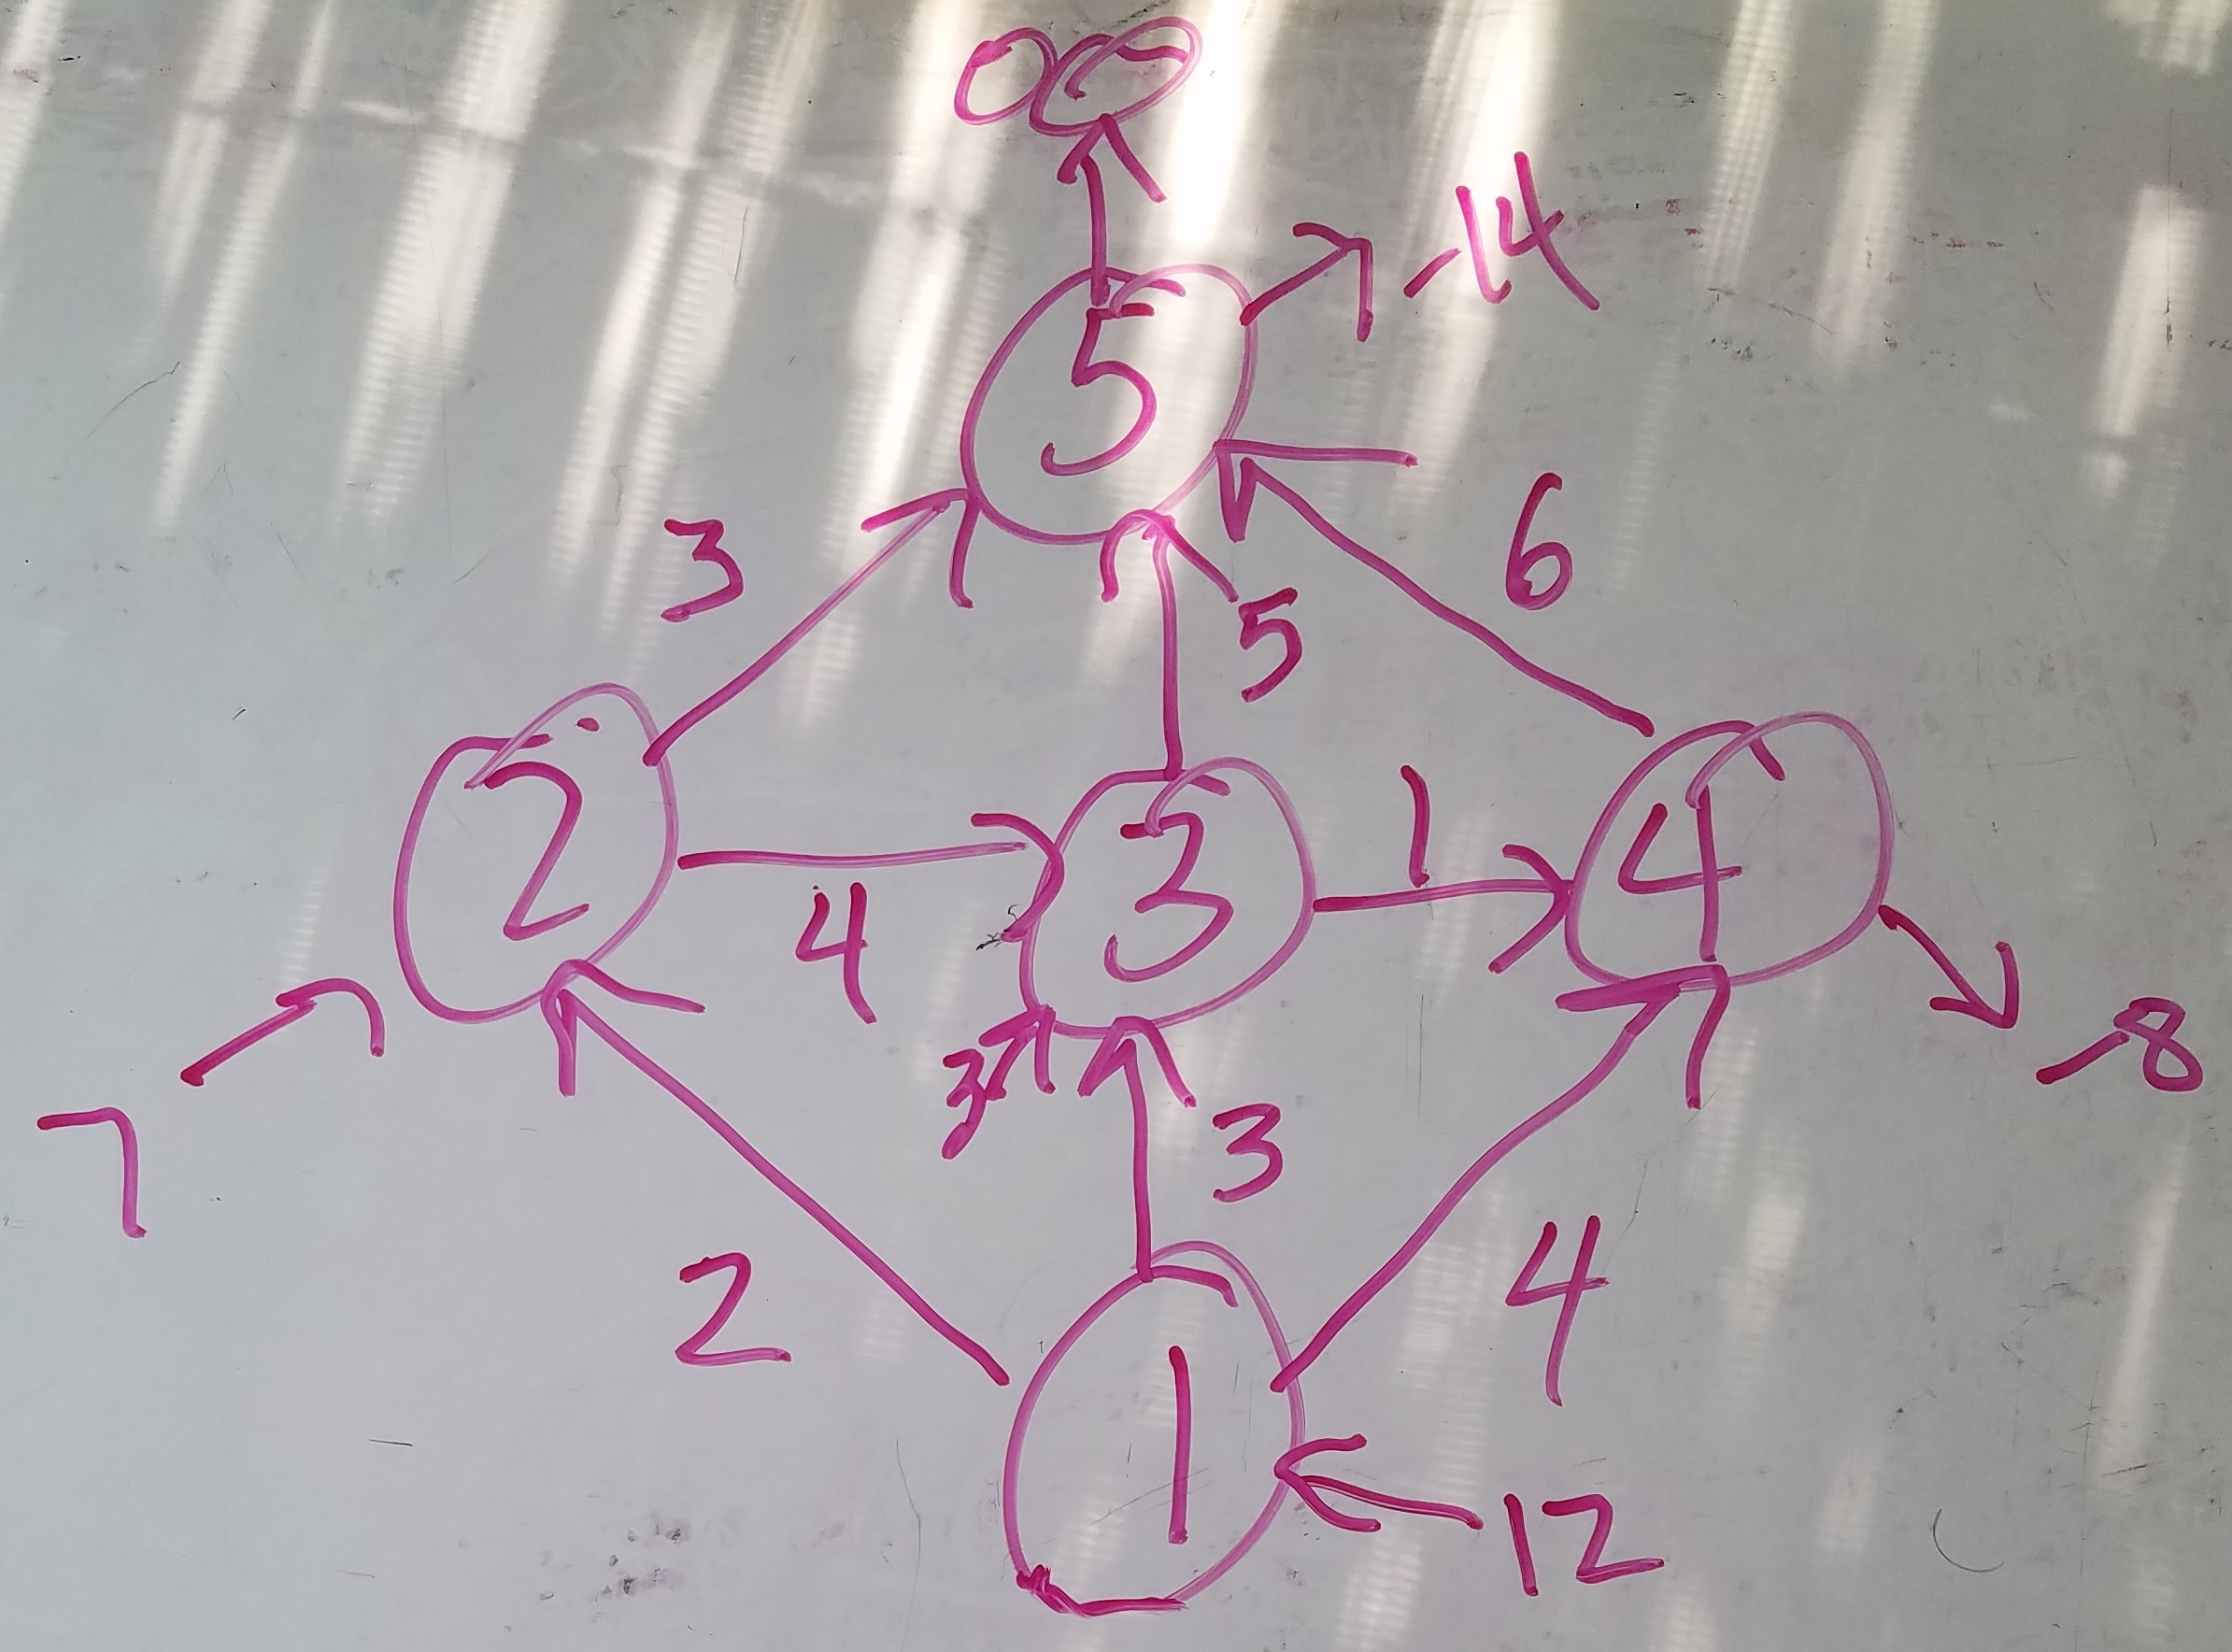
\includegraphics[width=0.6\textwidth]{lp5_2_cropped}
  \caption{This is the Flow Net}
\end{figure}

Starting Basic feasible soltuion T(N,A),where N=\{1,2,3,4,5\} and \\ $A=\{(1,3),(1,4),(2,3),(3,5),(5,\infty)\}$\\\\

\begin{figure}[h]
  \centering
  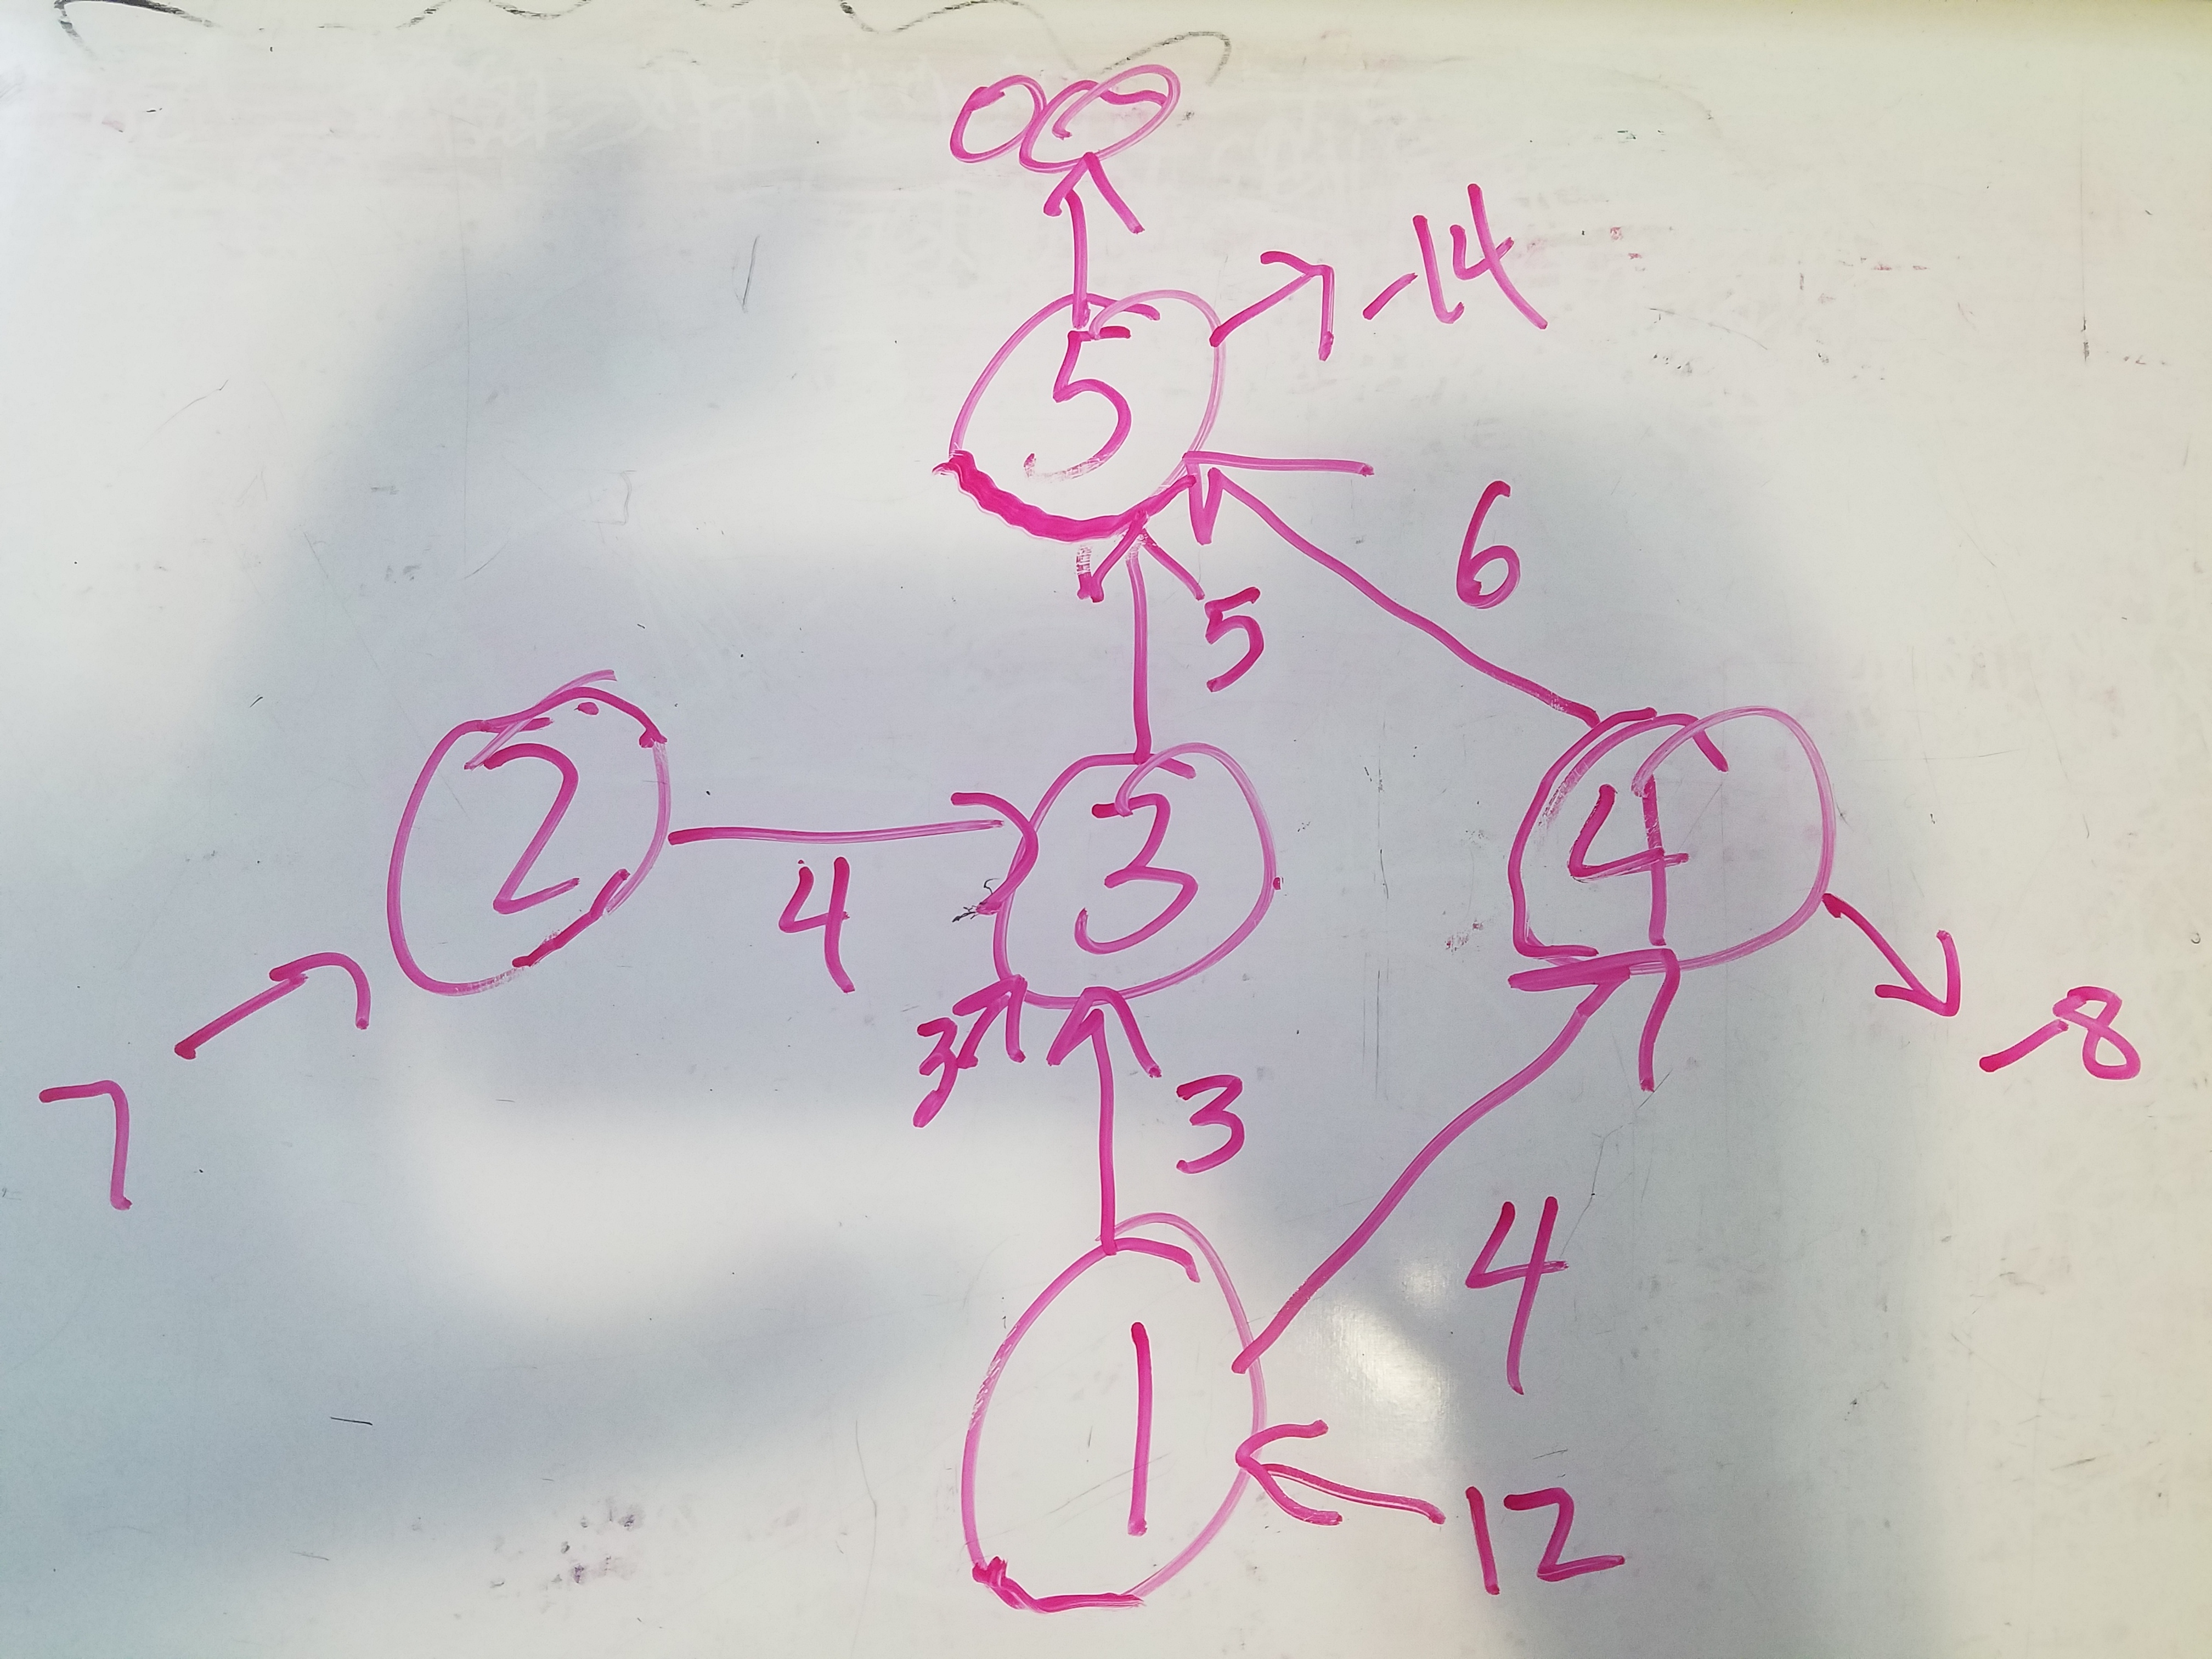
\includegraphics[width=0.6\textwidth]{lp5_2_feasible}
  \caption{This is the Rooted Spanning Tree}
\end{figure}
\begin{figure}[h]
  \centering
  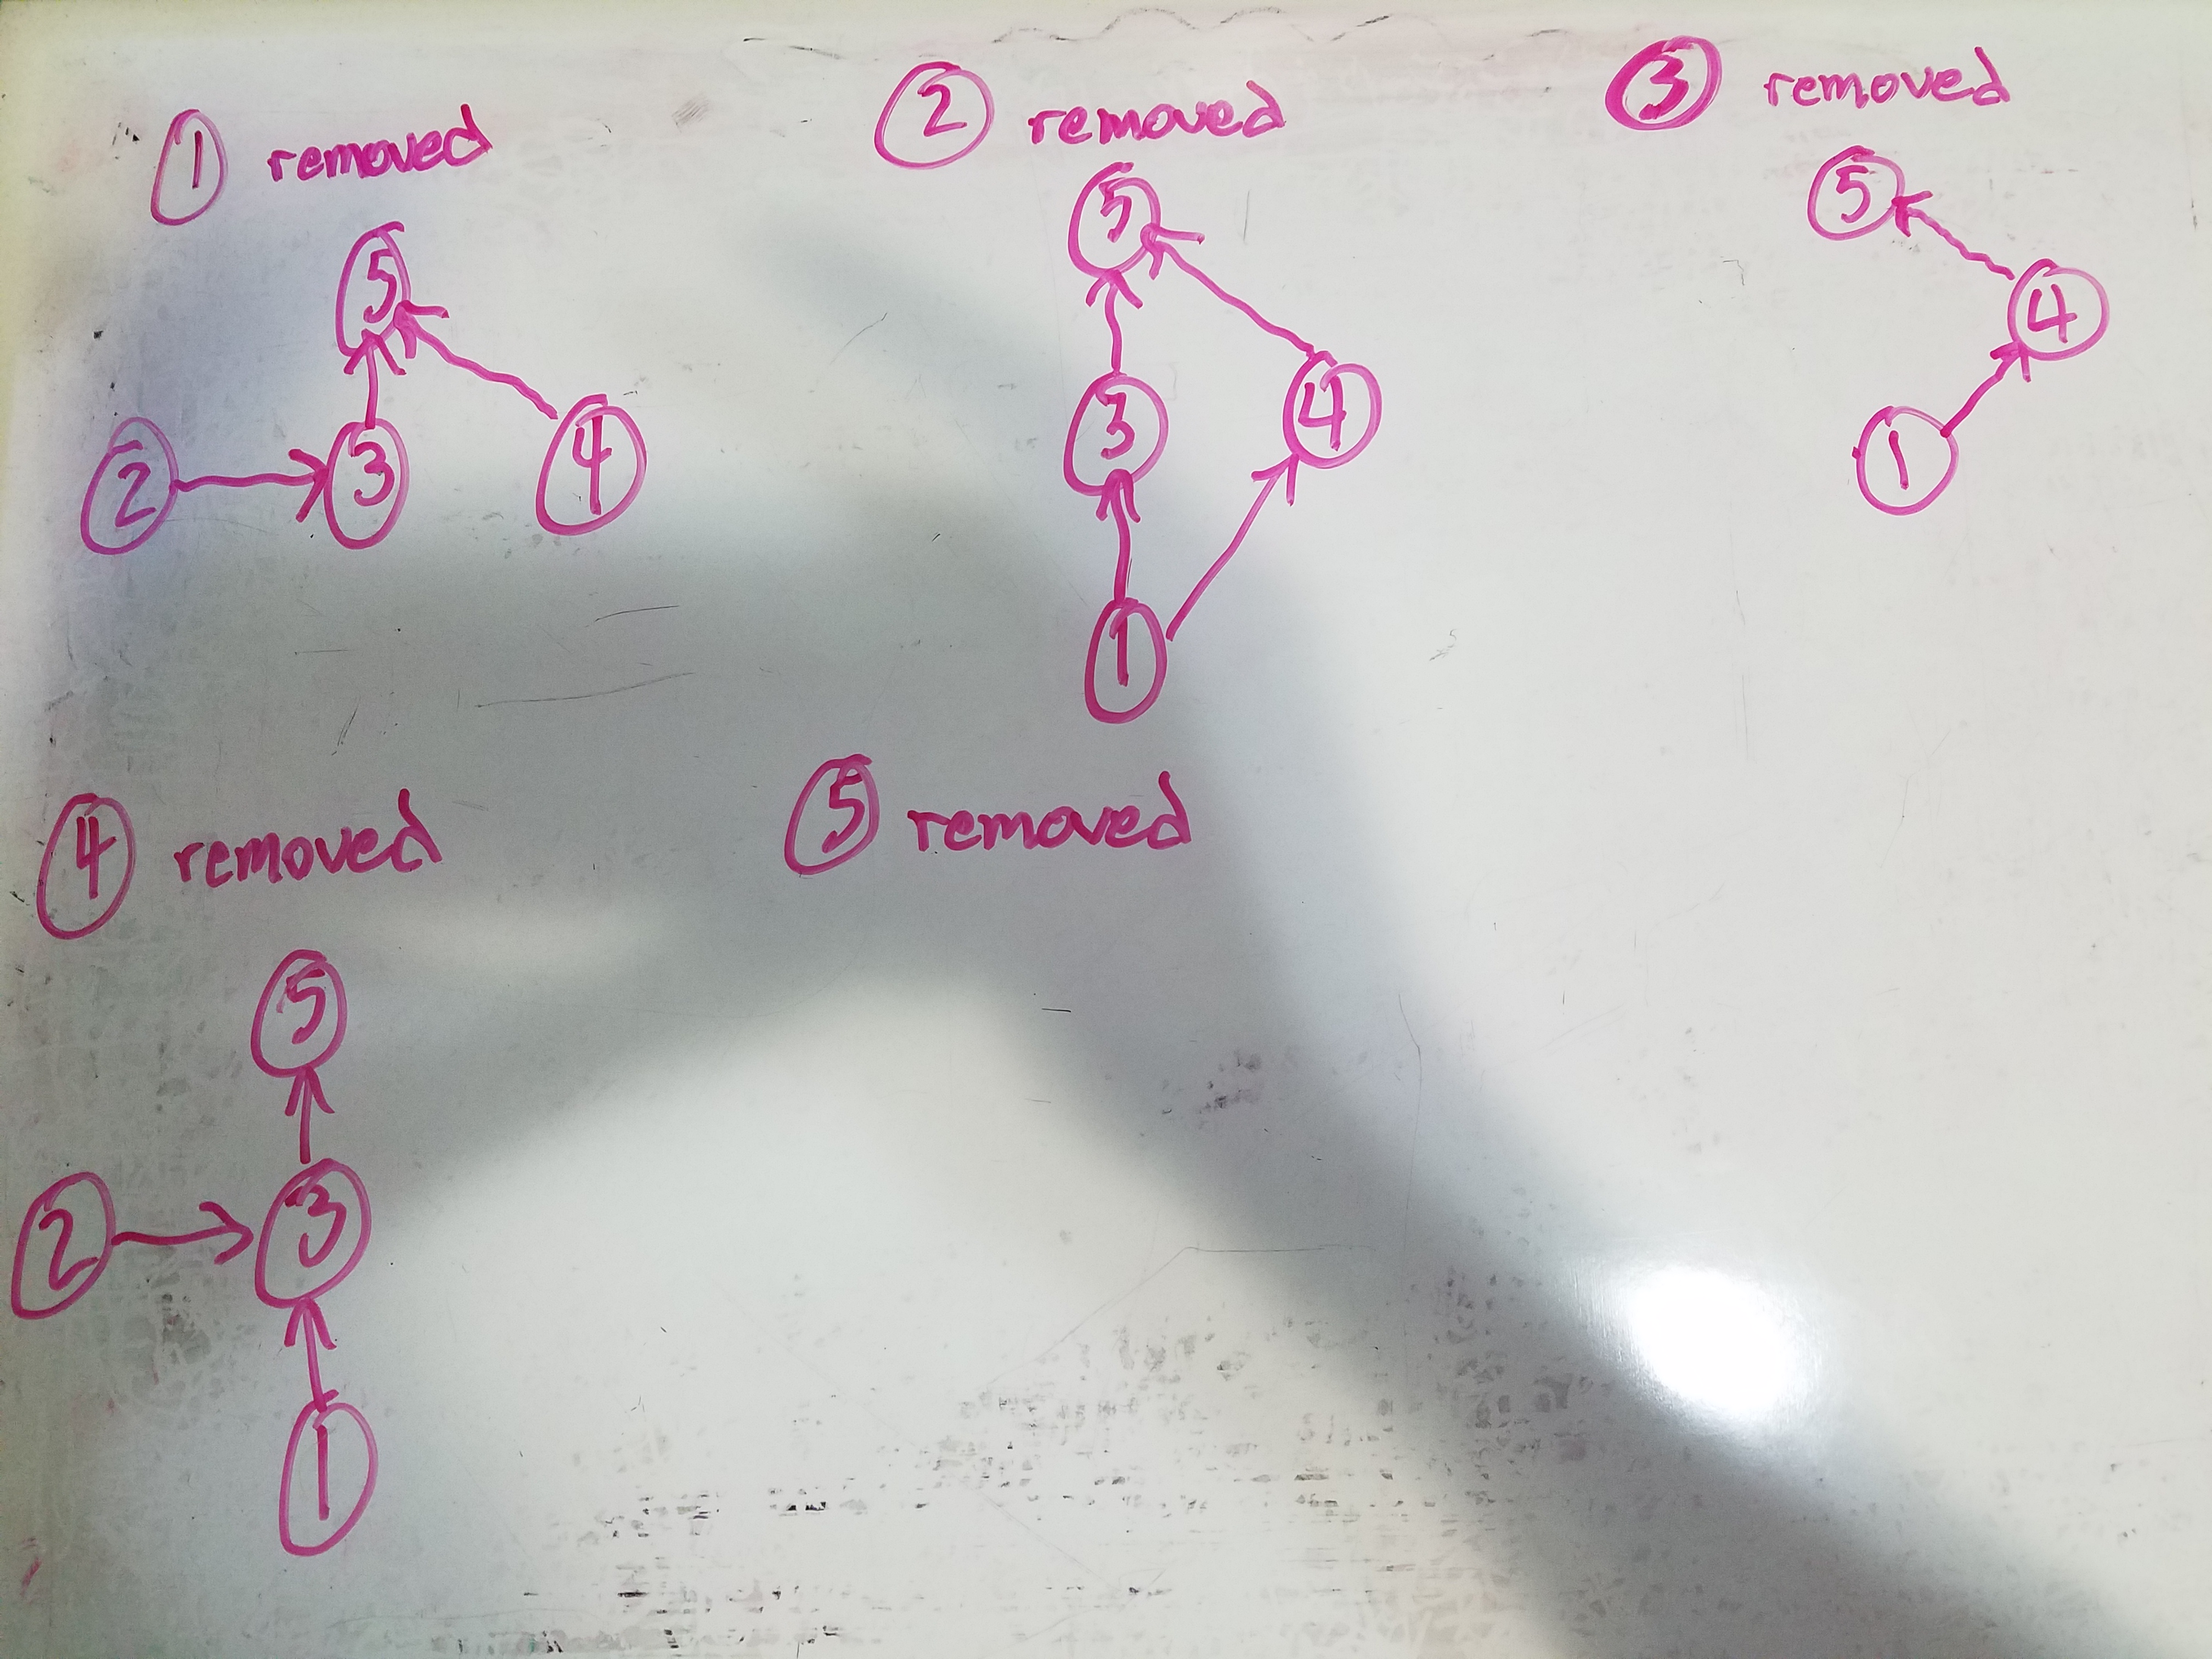
\includegraphics[width=0.6\textwidth]{lp5_2_removal}
  \caption{Removal Trees}
\end{figure}

$\begin{array}{r|rrrrrr}
      & (1,3) & (1,4) & (2,3) & (3,5) & (4,5) & Root Arc\\
    \hline
    1 & -1 & -1 & 0 & 0 & 0 & 0 \\
    2 & 0 & 0 & -1 & 0 & 0 & 0 \\
    3 & 1 & 0 & 1 & -1 & 0 & 0 \\
    4 & 0 & 1 & 0 & 0 & -1 & 0 \\
    5 & 0 & 0 & 0 & 0  & 1 & -1\\
\end{array}$

\begin{verbatim}
Results in:
x12 = 14
x13 = 40
x34 = 20
x25 = 88
z   = 27.0
\end{verbatim}

\newpage
\section{Source Code}
\subsection{NetSimplex.java}
\lstinputlisting[language=Java]{../../../Linear-And-Integer-Programming/src/main/java/assignment/NetSimplex.java}
\newpage
\subsection{MinimumSpanningTree.java}
\lstinputlisting[language=Java]{../../../Linear-And-Integer-Programming/src/main/java/utilities/spanningtree/MinimumSpanningTree.java}


\end{document}
